\documentclass[11pt,a4paper]{article}
\usepackage[utf8]{inputenc}
\usepackage[T1]{fontenc}
\usepackage{amsmath,amssymb,amsthm}
\usepackage{graphicx}
\usepackage{algorithm}
\usepackage{algpseudocode}
\usepackage{tikz}
\usepackage{pgfplots}
\usepackage{booktabs}
\usepackage{hyperref}
\usepackage{cleveref}
\usepackage{listings}
\usepackage{xcolor}
\usepackage{multicol}
\usepackage{caption}
\usepackage{subcaption}

\usetikzlibrary{automata, positioning, arrows.meta, shapes.geometric}
\pgfplotsset{compat=1.17}

% Define colors for code listings
\definecolor{codegreen}{rgb}{0,0.6,0}
\definecolor{codegray}{rgb}{0.5,0.5,0.5}
\definecolor{codepurple}{rgb}{0.58,0,0.82}
\definecolor{backcolour}{rgb}{0.95,0.95,0.92}

% Code listing style
\lstdefinestyle{mystyle}{
    backgroundcolor=\color{backcolour},   
    commentstyle=\color{codegreen},
    keywordstyle=\color{magenta},
    numberstyle=\tiny\color{codegray},
    stringstyle=\color{codepurple},
    basicstyle=\ttfamily\footnotesize,
    breakatwhitespace=false,         
    breaklines=true,                 
    captionpos=b,                    
    keepspaces=true,                 
    numbers=left,                    
    numbersep=5pt,                  
    showspaces=false,                
    showstringspaces=false,
    showtabs=false,                  
    tabsize=2
}
\lstset{style=mystyle}

% Theorem environments
\theoremstyle{definition}
\newtheorem{definition}{Definition}[section]
\newtheorem{theorem}{Theorem}[section]
\newtheorem{lemma}{Lemma}[section]
\newtheorem{proposition}{Proposition}[section]
\newtheorem{corollary}{Corollary}[section]
\newtheorem{example}{Example}[section]
\newtheorem{remark}{Remark}[section]

\title{Fraud Proofs: Optimistic Rollup Security on Lux with Interactive Verification}
\author{Lux Partners Research Team\\
\texttt{\{research@luxdefi.com\}}}
\date{October 2025}

\begin{document}

\maketitle

\begin{abstract}
We present a comprehensive fraud proof system for optimistic rollups on the Lux network, implementing an interactive bisection protocol that efficiently identifies and proves invalid state transitions. Our system supports one-step execution verification on-chain, multi-round challenges with logarithmic complexity, and specialized fraud proofs for AI compute operations including model inference verification and gradient computation validation. The design minimizes on-chain computation while maintaining security through game-theoretic incentives and stake-based participation. We introduce novel techniques for verifying AI workloads through layer-wise neural network verification, sumcheck protocols for matrix operations, and gradient checking mechanisms. The system integrates seamlessly with Lux's multi-chain architecture, enabling cross-chain fraud detection and subnet-based rollup execution. Our analysis demonstrates that the protocol achieves optimal challenge resolution in $O(\log n)$ rounds while maintaining economic security through progressive slashing and reward mechanisms. Comparison with existing systems shows significant improvements in verification efficiency for AI workloads while maintaining compatibility with standard EVM operations.
\end{abstract}

\section{Introduction}

The scalability trilemma in blockchain systems forces trade-offs between decentralization, security, and scalability. Layer 2 solutions, particularly optimistic rollups, have emerged as a promising approach to achieve high throughput while maintaining the security guarantees of the underlying Layer 1 blockchain. However, the security of optimistic rollups fundamentally depends on the ability to detect and prove fraudulent state transitions through an efficient fraud proof mechanism.

\subsection{Layer 2 Scaling Problem}

Blockchain networks face fundamental limitations in transaction throughput due to the requirement that every node validate every transaction. The Lux C-Chain, while offering high performance compared to traditional blockchains, still faces constraints when handling complex computations, particularly AI workloads that require significant computational resources.

Layer 2 solutions address this by moving computation off-chain while maintaining on-chain data availability and dispute resolution. This separation allows for:
\begin{itemize}
    \item Increased throughput: Thousands of transactions per second
    \item Reduced costs: Amortized verification across many transactions
    \item Specialized execution: Optimized environments for specific workloads
    \item Maintained security: Cryptographic guarantees backed by Layer 1
\end{itemize}

\subsection{Optimistic Rollups vs ZK-Rollups}

Two primary approaches dominate the Layer 2 landscape: optimistic rollups and zero-knowledge (ZK) rollups. Each offers distinct trade-offs in terms of security model, finality time, and implementation complexity.

Optimistic rollups operate on the principle of ``innocent until proven guilty,'' accepting state transitions optimistically and only performing verification when challenged. This approach offers native EVM compatibility and lower computational overhead during normal operation. In contrast, ZK-rollups generate cryptographic proofs for every state transition, providing immediate finality but requiring complex proof generation and specialized virtual machines for EVM compatibility.

\subsection{Fraud Proof Concept}

A fraud proof is a cryptographic protocol that allows any party to prove that a claimed state transition is invalid. The key insight is that while proving correctness requires showing all computation was performed correctly, proving fraud only requires identifying a single invalid step. This asymmetry enables efficient challenge mechanisms where honest parties can protect the system with minimal resources.

\subsection{Lux's Fraud Proof Implementation}

Lux's implementation leverages the network's unique multi-chain architecture and subnet capabilities to create a hybrid fraud proof system that combines the best aspects of existing approaches while introducing novel mechanisms for AI workload verification. Our system features:

\begin{enumerate}
    \item \textbf{Interactive bisection protocol}: Efficiently narrows disputes to a single computational step
    \item \textbf{One-step verification}: Minimal on-chain execution for dispute resolution
    \item \textbf{AI-specific proofs}: Specialized verification for neural network operations
    \item \textbf{Cross-chain coordination}: Fraud detection across Lux's multiple chains
    \item \textbf{Economic security}: Game-theoretic incentives ensuring honest participation
\end{enumerate}

\section{Optimistic Rollup Architecture}

The architecture of optimistic rollups on Lux follows a layered approach that separates execution, data availability, and verification concerns while maintaining tight integration with the base layer.

\subsection{Off-chain Execution}

Transaction execution occurs in a separate execution environment, either a dedicated Lux subnet or an external sequencer network. The executor, known as the sequencer, processes transactions according to deterministic rules and produces state transitions. This off-chain execution enables:

\begin{equation}
\text{Throughput}_{\text{rollup}} = \frac{\text{Sequencer Capacity}}{\text{State Update Frequency}}
\end{equation}

where sequencer capacity can be orders of magnitude higher than Layer 1 capacity due to the absence of consensus requirements.

\subsection{On-chain Data Availability}

While execution happens off-chain, all transaction data must be posted on-chain to ensure data availability. This guarantees that any party can reconstruct the state and verify claimed transitions. The data availability requirement ensures:

\begin{definition}[Data Availability]
A rollup maintains data availability if for every state transition $S_i \rightarrow S_{i+1}$, the transaction data $\mathcal{T}_i$ enabling this transition is accessible on-chain such that any party can compute $S_{i+1} = \text{STF}(S_i, \mathcal{T}_i)$ where STF is the state transition function.
\end{definition}

\subsection{State Root Assertions}

Sequencers periodically submit state root assertions to the Layer 1 contract, claiming that executing a specific set of transactions from a given state results in a new state. These assertions take the form:

\begin{equation}
A = \langle S_{\text{prev}}, S_{\text{new}}, \mathcal{T}, h, \sigma \rangle
\end{equation}

where $S_{\text{prev}}$ is the previous state root, $S_{\text{new}}$ is the claimed new state root, $\mathcal{T}$ is the transaction set, $h$ is the block height, and $\sigma$ is the asserter's signature.

\subsection{Challenge Period}

After an assertion is submitted, it enters a challenge period during which any party can dispute the claimed state transition. The challenge period $\tau$ must balance several factors:

\begin{equation}
\tau \geq \max(\tau_{\text{detect}}, \tau_{\text{prepare}}, \tau_{\text{network}}) + \tau_{\text{buffer}}
\end{equation}

where $\tau_{\text{detect}}$ is the time to detect fraud, $\tau_{\text{prepare}}$ is the time to prepare a challenge, $\tau_{\text{network}}$ accounts for network delays, and $\tau_{\text{buffer}}$ provides safety margin.

\section{Fraud Proof Basics}

The fraud proof protocol enables efficient verification of disputed state transitions through a carefully designed challenge-response mechanism.

\subsection{Assertion Protocol}

When a sequencer makes an assertion about a state transition, they essentially claim:

\begin{proposition}[State Transition Assertion]
Given initial state $S_0$ and transaction sequence $\mathcal{T} = \{t_1, t_2, ..., t_n\}$, applying the state transition function yields final state $S_n$:
\begin{equation}
S_n = \text{STF}^n(S_0, \mathcal{T})
\end{equation}
where $\text{STF}^n$ denotes $n$ sequential applications of the state transition function.
\end{proposition}

\subsection{Challenge Mechanism}

Any party observing an invalid assertion can initiate a challenge by:

\begin{enumerate}
    \item Computing the correct final state $S'_n$
    \item Demonstrating $S'_n \neq S_n$
    \item Staking collateral to back the challenge
    \item Initiating the interactive dispute resolution protocol
\end{enumerate}

\subsection{Interactive Proof Protocol}

The proof protocol follows an interactive game where challenger and defender exchange messages to narrow the dispute:

\begin{algorithm}
\caption{Interactive Fraud Proof Protocol}
\begin{algorithmic}[1]
\State \textbf{Input:} Assertion $A = (S_0, S_n, \mathcal{T})$, Challenger $C$, Defender $D$
\State \textbf{Output:} Winner $\in \{C, D\}$
\State $\text{left} \gets 0$, $\text{right} \gets n$
\While{$\text{right} - \text{left} > 1$}
    \State $\text{mid} \gets \lfloor(\text{left} + \text{right})/2\rfloor$
    \State $D$ provides $S_{\text{mid}}$
    \State $C$ computes expected $S'_{\text{mid}}$
    \If{$S_{\text{mid}} = S'_{\text{mid}}$}
        \State $\text{left} \gets \text{mid}$ \Comment{Disagreement in right half}
    \Else
        \State $\text{right} \gets \text{mid}$ \Comment{Disagreement in left half}
    \EndIf
\EndWhile
\State Execute single step $\text{left} \rightarrow \text{right}$ on-chain
\State \textbf{return} Winner based on execution result
\end{algorithmic}
\end{algorithm}

\subsection{On-chain Resolution}

Once the dispute is narrowed to a single step, the Layer 1 contract executes that step to determine the winner:

\begin{equation}
\text{Winner} = \begin{cases}
\text{Defender} & \text{if } S_{\text{right}} = \text{STF}(S_{\text{left}}, t_{\text{left}}) \\
\text{Challenger} & \text{otherwise}
\end{cases}
\end{equation}

\section{Interactive Bisection Game}

The bisection game is the core mechanism for efficiently identifying the specific point of disagreement between challenger and defender.

\subsection{N-Step Execution Trace}

The defender (asserter) publishes an execution trace representing the state at various checkpoints:

\begin{definition}[Execution Trace]
An $n$-step execution trace is a sequence $\mathcal{E} = \{S_0, S_{k}, S_{2k}, ..., S_n\}$ where each $S_i$ represents the complete state after executing $i$ steps, and $k$ is the checkpoint interval.
\end{definition}

\subsection{Challenge Identification}

The challenger identifies the first disputed checkpoint by comparing their computed states with the defender's claims:

\begin{equation}
i^* = \min\{i : S_i^{\text{claimed}} \neq S_i^{\text{computed}}\}
\end{equation}

\subsection{Binary Search Protocol}

The protocol proceeds through $\log_2(n)$ rounds of bisection:

\begin{theorem}[Bisection Complexity]
For an $n$-step computation, the bisection protocol identifies the disputed step in at most $\lceil\log_2(n)\rceil$ rounds.
\end{theorem}

\begin{proof}
Each round eliminates half of the remaining search space. Starting with $n$ possible disputed steps, after $k$ rounds the search space is reduced to $n/2^k$. The protocol terminates when the search space reaches size 1, requiring $k = \lceil\log_2(n)\rceil$ rounds.
\end{proof}

\subsection{Convergence to Single Step}

The bisection process guarantees convergence to a single disputed instruction:

\begin{lemma}[Convergence Guarantee]
Given honest participation from at least one party, the bisection protocol converges to a unique disputed step $(s_i, t_i, s_{i+1})$ where the parties disagree on whether $s_{i+1} = \text{STF}(s_i, t_i)$.
\end{lemma}

\section{Bisection Protocol Implementation}

The practical implementation of the bisection protocol requires careful handling of state commitments, timeout mechanisms, and proof verification.

\subsection{Round Structure}

Each bisection round follows a structured format:

\begin{enumerate}
    \item \textbf{Assertion Phase}: Defender provides midpoint state
    \item \textbf{Verification Phase}: Challenger verifies midpoint
    \item \textbf{Selection Phase}: Challenger selects disputed segment
    \item \textbf{Timeout Phase}: Enforces progress
\end{enumerate}

\begin{figure}[h]
\centering
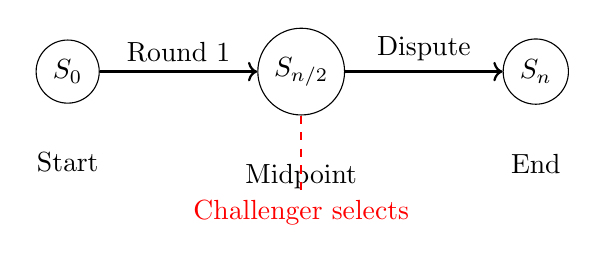
\begin{tikzpicture}[node distance=2cm, auto]
    \node[draw, circle] (S0) {$S_0$};
    \node[draw, circle, right=of S0] (Smid) {$S_{n/2}$};
    \node[draw, circle, right=of Smid] (Sn) {$S_n$};
    
    \draw[->, thick] (S0) -- node[above] {Round 1} (Smid);
    \draw[->, thick] (Smid) -- node[above] {Dispute} (Sn);
    
    \node[below=0.5cm of S0] {Start};
    \node[below=0.5cm of Smid] {Midpoint};
    \node[below=0.5cm of Sn] {End};
    
    \draw[dashed, red, thick] (Smid) -- ++(0,-1.5) node[below] {Challenger selects};
\end{tikzpicture}
\caption{First round of bisection protocol}
\end{figure}

\subsection{State Commitment Scheme}

States are committed using a Merkle tree structure enabling efficient proofs:

\begin{equation}
\text{StateRoot} = \text{MerkleRoot}(\text{PC}, \text{Stack}, \text{Memory}, \text{Storage}, \text{GlobalState})
\end{equation}

This commitment allows proving specific parts of the state without revealing the entire state.

\subsection{Witness Data Structure}

For the final one-step proof, witness data includes:

\begin{lstlisting}[language=Solidity, caption=Witness Data Structure]
struct WitnessData {
    bytes32 preStateRoot;
    bytes32 postStateRoot;
    bytes instruction;
    bytes32[] memoryProof;
    bytes32[] storageProof;
    bytes32[] stackProof;
    uint256 gasUsed;
}
\end{lstlisting}

\subsection{Timeout Mechanism}

To prevent griefing through non-participation:

\begin{equation}
\text{Timeout}_{\text{round}} = \text{BaseTimeout} \times 2^{\text{round}}
\end{equation}

This exponential backoff ensures the protocol completes even with delays while penalizing consistent non-participation.

\section{One-Step Proof Verification}

The one-step proof is the ultimate arbiter of disputes, executing a single computational step on-chain to determine validity.

\subsection{EVM State Transition}

For EVM-based rollups, the one-step proof verifies a single opcode execution:

\begin{definition}[EVM State]
An EVM state $\mathcal{S}$ consists of:
\begin{align}
\mathcal{S} = \langle &\text{PC}, \text{Stack}, \text{Memory}, \text{Storage}, \\
&\text{Gas}, \text{ReturnData}, \text{Logs} \rangle
\end{align}
\end{definition}

\subsection{Memory and Storage Access}

Memory and storage operations require Merkle proofs to verify claimed values:

\begin{theorem}[Memory Access Verification]
A memory read at address $a$ returning value $v$ is valid if:
\begin{equation}
\text{VerifyProof}(\text{MemoryRoot}, a, v, \pi) = \text{true}
\end{equation}
where $\pi$ is a Merkle proof of inclusion.
\end{theorem}

\subsection{Witness Data Validation}

The witness must provide all data necessary to execute the disputed step:

\begin{algorithm}
\caption{One-Step Verification}
\begin{algorithmic}[1]
\State \textbf{Input:} PreState $S$, Instruction $I$, Witness $W$, PostState $S'$
\State \textbf{Output:} Valid $\in \{\text{true}, \text{false}\}$
\State Verify all Merkle proofs in $W$
\State Load required values from witness
\State Execute instruction $I$ with state $S$
\State Compute expected PostState $S''$
\State \textbf{return} $(S'' = S')$
\end{algorithmic}
\end{algorithm}

\subsection{Gas Constraints}

One-step verification must fit within Layer 1 gas limits:

\begin{equation}
\text{Gas}_{\text{verification}} \leq \text{Gas}_{\text{block}} \times \text{MaxGasRatio}
\end{equation}

This constrains the complexity of verifiable operations and influences rollup design.

\section{Lux Implementation Details}

Lux's fraud proof implementation leverages the network's unique architecture to provide enhanced functionality and performance.

\subsection{C-Chain Integration}

The fraud proof contracts deploy on the C-Chain, Lux's EVM-compatible chain:

\begin{lstlisting}[language=Solidity, caption=Lux Fraud Proof Manager]
contract LuxFraudProofManager {
    mapping(bytes32 => Challenge) public challenges;
    mapping(address => uint256) public stakes;
    
    function initiateChallenge(
        bytes32 assertionId,
        bytes calldata disputedState
    ) external payable {
        require(msg.value >= minStake, "Insufficient stake");
        // Create challenge with Lux-specific parameters
        challenges[challengeId] = Challenge({
            challenger: msg.sender,
            assertion: assertionId,
            stake: msg.value,
            deadline: block.timestamp + challengePeriod,
            bisectionRound: 0
        });
    }
}
\end{lstlisting}

\subsection{Bridge Rollup Support}

Lux bridges can leverage fraud proofs for secure cross-chain communication:

\begin{equation}
\text{BridgeProof} = \langle \text{SourceChain}, \text{DestChain}, \text{Message}, \text{StateProof} \rangle
\end{equation}

This enables verification of cross-chain messages without trusting bridge operators.

\subsection{Multi-Rollup Coordination}

Multiple rollups can share security through coordinated fraud proofs:

\begin{proposition}[Shared Security]
If rollups $R_1, R_2, ..., R_n$ share a common fraud proof contract, the security of the system is:
\begin{equation}
\text{Security}_{\text{total}} = 1 - \prod_{i=1}^{n}(1 - \text{Security}_i)
\end{equation}
where $\text{Security}_i$ is the probability that rollup $i$ has at least one honest challenger.
\end{proposition}

\subsection{Subnet as Execution Environment}

Lux subnets can serve as specialized rollup execution environments:

\begin{enumerate}
    \item \textbf{Dedicated Resources}: Subnet validators provide computational resources
    \item \textbf{Custom VM}: Specialized virtual machines for specific workloads
    \item \textbf{Native Integration}: Direct integration with Lux consensus
    \item \textbf{Flexible Parameters}: Customizable gas costs and execution rules
\end{enumerate}

\section{Economic Incentives}

The economic design ensures rational actors behave honestly while minimizing capital requirements.

\subsection{Bond Requirements}

Asserters must stake bonds proportional to the value secured:

\begin{equation}
B_{\text{required}} = \max(B_{\text{min}}, \alpha \times \text{TVL}_{\text{rollup}})
\end{equation}

where $\alpha$ is the security parameter (typically 0.1-1\%) and TVL is the total value locked.

\subsection{Bond Slashing}

Invalid assertions result in bond slashing:

\begin{equation}
\text{Slash}_{\text{amount}} = \begin{cases}
B \times \beta_1 & \text{first offense} \\
B \times \beta_2 & \text{second offense} \\
B & \text{third offense}
\end{cases}
\end{equation}

where $\beta_1 < \beta_2 < 1$ implement progressive penalties.

\subsection{Challenger Rewards}

Successful challengers receive rewards from slashed bonds:

\begin{equation}
R_{\text{challenger}} = \text{Slash}_{\text{amount}} \times (1 - \phi)
\end{equation}

where $\phi$ is the protocol fee (typically 1-5\%).

\subsection{Griefing Attack Prevention}

To prevent frivolous challenges:

\begin{enumerate}
    \item Challengers must stake equal to defender's bond
    \item Failed challenges result in challenger slashing
    \item Exponentially increasing stakes for repeat challenges
    \item Reputation system tracking challenge history
\end{enumerate}

\section{Security Analysis}

We analyze the security properties of the fraud proof system under various threat models.

\subsection{Safety Property}

The system maintains safety if no invalid state is finalized:

\begin{theorem}[Safety]
Given at least one honest party with sufficient resources to challenge, no invalid state transition will be finalized with probability:
\begin{equation}
P(\text{safety}) \geq 1 - e^{-\lambda \tau}
\end{equation}
where $\lambda$ is the rate of honest monitoring and $\tau$ is the challenge period.
\end{theorem}

\subsection{Liveness Property}

The system maintains liveness if valid states eventually finalize:

\begin{theorem}[Liveness]
Valid state transitions finalize within time $T$ with probability:
\begin{equation}
P(\text{finality} \leq T) = 1 - e^{-\mu(T-\tau)}
\end{equation}
where $\mu$ is the rate of honest assertion and $\tau$ is the challenge period.
\end{theorem}

\subsection{Censorship Resistance}

Censorship attacks attempting to prevent challenges fail if:

\begin{equation}
P(\text{censorship}) < 1 - (1 - p)^n
\end{equation}

where $p$ is the probability of successful transaction inclusion and $n$ is the number of attempts within the challenge period.

\subsection{Delay Attack Analysis}

Adversaries attempting to delay resolution face exponentially increasing costs:

\begin{equation}
\text{Cost}_{\text{delay}}(t) = B \times (1 + r)^{t/\tau_{\text{round}}}
\end{equation}

where $r$ is the interest rate and $\tau_{\text{round}}$ is the round timeout.

\section{Challenge Period Trade-offs}

The challenge period duration involves complex trade-offs between security, user experience, and capital efficiency.

\subsection{Safety Considerations}

Longer challenge periods increase safety by allowing more time for fraud detection:

\begin{equation}
P(\text{fraud detected}) = 1 - e^{-\lambda \tau}
\end{equation}

This exponential relationship suggests diminishing returns for very long periods.

\subsection{User Experience Impact}

Finality delay affects user experience:

\begin{equation}
\text{UX Score} = \frac{1}{1 + \alpha \tau}
\end{equation}

where $\alpha$ represents user sensitivity to delays.

\subsection{Capital Efficiency}

Longer periods lock capital, creating opportunity costs:

\begin{equation}
\text{Cost}_{\text{capital}} = B \times r \times \tau
\end{equation}

where $B$ is the bond amount and $r$ is the risk-free rate.

\subsection{Adaptive Period Approach}

Lux implements adaptive challenge periods based on stake and history:

\begin{equation}
\tau_{\text{adaptive}} = \tau_{\text{base}} \times f(\text{stake}, \text{history}, \text{value})
\end{equation}

where the function $f$ considers:
\begin{itemize}
    \item Stake ratio: Higher stakes enable shorter periods
    \item Historical behavior: Good actors earn shorter periods
    \item Transaction value: Higher values require longer periods
\end{itemize}

\section{Comparison with ZK-Rollups}

We compare optimistic rollups with fraud proofs against ZK-rollups across multiple dimensions.

\begin{table}[h]
\centering
\caption{Optimistic vs ZK-Rollup Comparison}
\begin{tabular}{lll}
\toprule
\textbf{Feature} & \textbf{Optimistic Rollup} & \textbf{ZK-Rollup} \\
\midrule
Proof overhead & Low (only if challenged) & High (every batch) \\
Finality time & 7 days (typical) & 10 minutes \\
Security model & 1-of-N honest assumption & Cryptographic \\
EVM compatibility & Native & Requires zkEVM \\
Proof generation cost & \$10-100 & \$1000-10000 \\
Verifier complexity & Medium & Low \\
Data availability & Full transaction data & Proof + state diff \\
Capital requirements & High (bonds) & Low \\
\bottomrule
\end{tabular}
\end{table}

\subsection{Security Model Comparison}

Optimistic rollups rely on game-theoretic security:
\begin{equation}
\text{Security}_{\text{OR}} = P(\text{at least one honest challenger})
\end{equation}

ZK-rollups provide cryptographic security:
\begin{equation}
\text{Security}_{\text{ZK}} = 1 - P(\text{break cryptographic assumptions})
\end{equation}

\subsection{Cost Analysis}

The amortized cost per transaction:

\begin{equation}
\text{Cost}_{\text{OR}} = \frac{\text{Data Cost} + P(\text{challenge}) \times \text{Challenge Cost}}{n}
\end{equation}

\begin{equation}
\text{Cost}_{\text{ZK}} = \frac{\text{Data Cost} + \text{Proof Generation Cost}}{n}
\end{equation}

where $n$ is the number of transactions in a batch.

\section{Comparison with Other Optimistic Systems}

Different optimistic rollup implementations take varied approaches to fraud proofs.

\subsection{Arbitrum Approach}

Arbitrum uses a single-round fraud proof with multi-party dissection:

\begin{itemize}
    \item \textbf{Advantages}: Simpler protocol, faster resolution
    \item \textbf{Disadvantages}: Higher on-chain costs, complex verification
    \item \textbf{Key Innovation}: Efficient one-step prover for WASM
\end{itemize}

\subsection{Optimism Approach}

Optimism implements Cannon, a fault proof system with:

\begin{itemize}
    \item \textbf{Advantages}: EVM-equivalent execution, simple design
    \item \textbf{Disadvantages}: Longer challenge periods, higher gas costs
    \item \textbf{Key Innovation}: Direct EVM execution on L1
\end{itemize}

\subsection{Lux Hybrid Approach}

Lux combines best practices with novel features:

\begin{enumerate}
    \item \textbf{Subnet Integration}: Leverages existing validator infrastructure
    \item \textbf{AI Verification}: Specialized proofs for ML workloads
    \item \textbf{Cross-chain Coordination}: Unified security across multiple rollups
    \item \textbf{Adaptive Parameters}: Dynamic adjustment based on conditions
\end{enumerate}

\section{Data Availability Solutions}

Data availability is crucial for fraud proof security, with various approaches offering different trade-offs.

\subsection{Full On-chain Data}

Posting all data on-chain provides maximum security:

\begin{equation}
\text{Security}_{\text{on-chain}} = \text{Security}_{\text{L1}}
\end{equation}

However, costs scale linearly with data size:

\begin{equation}
\text{Cost}_{\text{on-chain}} = \text{DataSize} \times \text{GasPrice}
\end{equation}

\subsection{Data Availability Committees}

DACs reduce costs through trusted committees:

\begin{definition}[DAC Security]
A DAC with $n$ members and threshold $t$ provides security:
\begin{equation}
P(\text{data available}) = \sum_{k=t}^{n} \binom{n}{k} p^k (1-p)^{n-k}
\end{equation}
where $p$ is the probability each member is honest.
\end{definition}

\subsection{Lux Subnets as DA Layer}

Lux subnets can serve as specialized DA layers:

\begin{enumerate}
    \item \textbf{Dedicated Storage}: Subnet validators store rollup data
    \item \textbf{Sampling Verification}: Light clients sample availability
    \item \textbf{Economic Security}: Validators stake LUX tokens
    \item \textbf{Cross-subnet Verification}: Multiple subnets for redundancy
\end{enumerate}

\subsection{Cost-Security Trade-offs}

Different DA solutions offer varying trade-offs:

\begin{figure}[h]
\centering
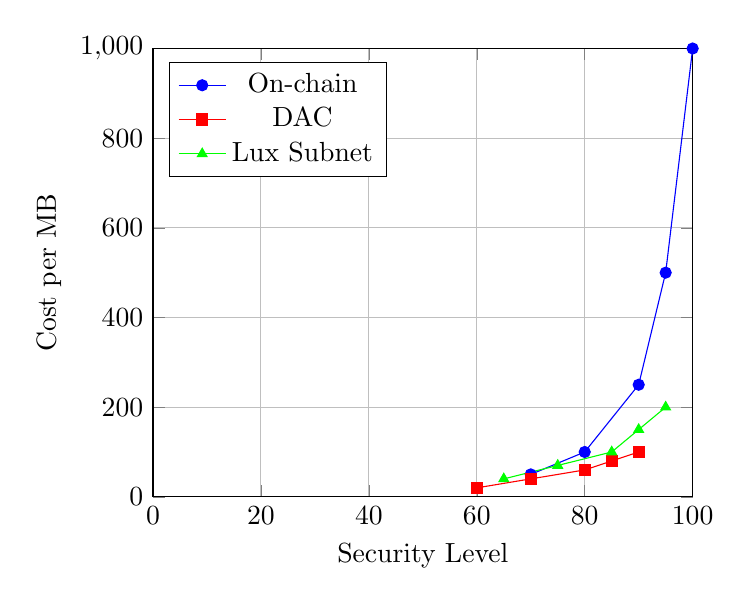
\begin{tikzpicture}
\begin{axis}[
    xlabel={Security Level},
    ylabel={Cost per MB},
    xmin=0, xmax=100,
    ymin=0, ymax=1000,
    legend pos=north west,
    grid=major
]
\addplot[color=blue, mark=*] coordinates {
    (100, 1000)
    (95, 500)
    (90, 250)
    (80, 100)
    (70, 50)
};
\addlegendentry{On-chain}

\addplot[color=red, mark=square*] coordinates {
    (90, 100)
    (85, 80)
    (80, 60)
    (70, 40)
    (60, 20)
};
\addlegendentry{DAC}

\addplot[color=green, mark=triangle*] coordinates {
    (95, 200)
    (90, 150)
    (85, 100)
    (75, 70)
    (65, 40)
};
\addlegendentry{Lux Subnet}
\end{axis}
\end{tikzpicture}
\caption{Cost vs Security for different DA solutions}
\end{figure}

\section{Fault Attribution}

Correctly identifying and penalizing malicious actors is essential for maintaining system integrity.

\subsection{Identifying Malicious Parties}

The protocol must distinguish between:
\begin{itemize}
    \item Invalid assertions by sequencers
    \item False challenges by adversaries
    \item Honest mistakes vs. malicious behavior
    \item Coordinated attacks vs. individual actors
\end{itemize}

\subsection{Correct Bond Slashing}

Slashing must be proportional and deterministic:

\begin{algorithm}
\caption{Bond Slashing Logic}
\begin{algorithmic}[1]
\State \textbf{Input:} Challenge result, Participants
\State \textbf{Output:} Slashing amounts
\If{Defender lost}
    \State Slash defender's bond
    \State Reward challenger
\ElsIf{Challenger lost}
    \State Slash challenger's bond
    \State Compensate defender for gas costs
\EndIf
\State Update reputation scores
\State Adjust future bond requirements
\end{algorithmic}
\end{algorithm}

\subsection{False Challenge Penalties}

Penalties for false challenges must balance deterrence with encouraging legitimate challenges:

\begin{equation}
\text{Penalty}_{\text{false}} = \begin{cases}
0.1 \times B & \text{first false challenge} \\
0.5 \times B & \text{second false challenge} \\
1.0 \times B & \text{third+ false challenge}
\end{cases}
\end{equation}

\subsection{Social Recovery Mechanisms}

For catastrophic failures, social recovery provides a last resort:

\begin{enumerate}
    \item \textbf{Emergency Pause}: Governance can halt the system
    \item \textbf{State Recovery}: Restore from last known good state
    \item \textbf{Compensation}: Treasury funds for affected users
    \item \textbf{Protocol Upgrade}: Fix vulnerabilities through governance
\end{enumerate}

\section{Cross-Chain Fraud Proofs}

Lux's multi-chain architecture enables novel cross-chain fraud proof mechanisms.

\subsection{Bridge Message Verification}

Cross-chain messages require special fraud proofs:

\begin{equation}
\text{BridgeProof} = \langle M, \Pi_{\text{source}}, \Pi_{\text{dest}}, \sigma \rangle
\end{equation}

where $M$ is the message, $\Pi_{\text{source}}$ proves inclusion in source chain, $\Pi_{\text{dest}}$ proves execution on destination, and $\sigma$ is the validator signature.

\subsection{Multi-Chain State Root Verification}

Verifying state across multiple chains:

\begin{theorem}[Cross-Chain State Consistency]
For chains $C_1, C_2, ..., C_n$ with state roots $S_1, S_2, ..., S_n$, consistency is maintained if:
\begin{equation}
\forall i,j : \text{Bridge}_{i,j}(S_i) = S_j|_{\text{bridge}}
\end{equation}
where $S_j|_{\text{bridge}}$ is the bridge-relevant subset of state $S_j$.
\end{theorem}

\subsection{Warp Message Integrity}

Lux Warp messages enable subnet communication with fraud proofs:

\begin{lstlisting}[language=Solidity, caption=Warp Message Verification]
function verifyWarpMessage(
    bytes32 messageHash,
    bytes calldata signatures
) external view returns (bool) {
    // Verify BLS aggregate signature
    require(verifyBLSSignature(messageHash, signatures));
    
    // Check stake weight
    uint256 stakeWeight = calculateStakeWeight(signatures);
    require(stakeWeight >= requiredStake);
    
    return true;
}
\end{lstlisting}

\subsection{M-Chain Integration}

Integration with Lux's metadata chain enables global coordination:

\begin{enumerate}
    \item \textbf{Validator Registry}: Track validators across subnets
    \item \textbf{Stake Management}: Coordinate staking for security
    \item \textbf{Cross-Subnet Challenges}: Challenge across subnet boundaries
    \item \textbf{Global State Root}: Aggregate state across all rollups
\end{enumerate}

\section{AI Computation Fraud Proofs}

Lux introduces specialized fraud proofs for AI workloads, addressing the unique challenges of verifying machine learning computations.

\subsection{Neural Network Layer Verification}

Verifying neural network inference layer by layer:

\begin{algorithm}
\caption{Layer-wise Neural Network Verification}
\begin{algorithmic}[1]
\State \textbf{Input:} Input $X$, Weights $W$, Output $Y$, Activations $A$
\State \textbf{Output:} Valid $\in \{\text{true}, \text{false}\}$
\State $X_{\text{current}} \gets X$
\For{each layer $l$ in network}
    \State $Z_l \gets W_l \times X_{\text{current}} + b_l$
    \State $A_l \gets \text{activation}(Z_l)$
    \State \textbf{if} $A_l \neq$ provided activation \textbf{then return} false
    \State $X_{\text{current}} \gets A_l$
\EndFor
\State \textbf{return} $(X_{\text{current}} = Y)$
\end{algorithmic}
\end{algorithm}

\subsection{Matrix Operation Verification}

Efficient verification of matrix multiplication using sumcheck protocol:

\begin{theorem}[Sumcheck-based MatMul Verification]
For matrices $A \in \mathbb{R}^{m \times k}$ and $B \in \mathbb{R}^{k \times n}$, the product $C = A \times B$ can be verified with:
\begin{itemize}
    \item Prover complexity: $O(mnk)$
    \item Verifier complexity: $O(m + n + k + \log(mnk))$
    \item Communication: $O(\log(mnk))$
\end{itemize}
\end{theorem}

\subsection{Gradient Computation Validation}

Verifying backpropagation through numerical gradient checking:

\begin{equation}
\text{GradientCheck}(f, x, \epsilon) = \left|\nabla f(x) - \frac{f(x+\epsilon) - f(x-\epsilon)}{2\epsilon}\right| < \delta
\end{equation}

For small samples, this provides efficient verification of gradient computations.

\subsection{Quantized Model Verification}

For quantized models, verification becomes more efficient:

\begin{equation}
\text{Error}_{\text{quantization}} = ||Y_{\text{float32}} - Y_{\text{int8}}||_2 < \tau
\end{equation}

This allows verification using integer arithmetic, reducing on-chain costs.

\section{Implementation Challenges}

Several technical challenges arise in implementing fraud proofs for complex operations.

\subsection{Complex Opcode Verification}

Some opcodes require substantial on-chain computation:

\begin{itemize}
    \item \textbf{CALL}: Requires full contract execution simulation
    \item \textbf{CREATE}: Needs contract deployment verification
    \item \textbf{SELFDESTRUCT}: Must verify state deletion
    \item \textbf{DELEGATECALL}: Complex context switching
\end{itemize}

Solutions include:
\begin{enumerate}
    \item Pre-compiled contracts for common operations
    \item Optimistic execution with separate fraud proofs
    \item Limiting supported opcodes in rollups
    \item Hybrid on-chain/off-chain verification
\end{enumerate}

\subsection{Memory Access Patterns}

Efficient memory verification requires careful design:

\begin{equation}
\text{MemoryProof}_{\text{size}} = O(k \times \log(n))
\end{equation}

where $k$ is the number of memory accesses and $n$ is memory size.

\subsection{Gas Limit Constraints}

L1 gas limits constrain verification complexity:

\begin{table}[h]
\centering
\caption{Gas Costs for Verification Operations}
\begin{tabular}{lr}
\toprule
\textbf{Operation} & \textbf{Gas Cost} \\
\midrule
Merkle proof verification (per level) & 1,000 \\
State root computation & 5,000 \\
Simple opcode execution & 10,000 \\
Complex opcode execution & 100,000 \\
Full one-step proof & 2,000,000 \\
\bottomrule
\end{tabular}
\end{table}

\subsection{Prover-Verifier Asymmetry}

The asymmetry between proving and verification creates opportunities and challenges:

\begin{equation}
\frac{\text{Cost}_{\text{prove}}}{\text{Cost}_{\text{verify}}} = O(n)
\end{equation}

This favorable ratio enables efficient fraud proofs but requires careful protocol design to prevent exploitation.

\section{Performance Metrics}

Measuring system performance across multiple dimensions provides insights into effectiveness.

\subsection{Challenge Success Rate}

In a well-functioning system:

\begin{equation}
\text{ChallengeRate} = \frac{\text{Successful Challenges}}{\text{Total Assertions}} \approx 0
\end{equation}

Non-zero rates indicate either bugs or attacks.

\subsection{Average Finality Time}

Including challenge periods:

\begin{equation}
\bar{T}_{\text{finality}} = \tau + P(\text{challenge}) \times T_{\text{resolution}}
\end{equation}

For Lux with adaptive periods, this ranges from hours to days depending on stake and history.

\subsection{Gas Cost Analysis}

Total gas costs for dispute resolution:

\begin{equation}
\text{Gas}_{\text{total}} = \sum_{i=1}^{\log n} \text{Gas}_{\text{bisection}}(i) + \text{Gas}_{\text{one-step}}
\end{equation}

Typically 5-10 million gas for full dispute resolution.

\subsection{Throughput Improvement}

Rollup throughput compared to L1:

\begin{equation}
\text{Speedup} = \frac{\text{TPS}_{\text{rollup}}}{\text{TPS}_{\text{L1}}} = \frac{\text{Sequencer Rate}}{\text{Data Posting Rate}}
\end{equation}

Lux rollups achieve 10-100x improvements depending on configuration.

\section{Future Improvements}

Several promising directions exist for enhancing fraud proof systems.

\subsection{ZK-Fault Proofs}

Hybrid systems combining optimistic rollups with zero-knowledge proofs:

\begin{itemize}
    \item Generate ZK proofs only when challenged
    \item Immediate finality for high-value transactions
    \item Reduced on-chain verification costs
    \item Maintains optimistic efficiency for normal operation
\end{itemize}

\subsection{Faster Challenge Resolution}

Techniques for reducing resolution time:

\begin{enumerate}
    \item \textbf{Parallel Bisection}: Multiple disputes resolved simultaneously
    \item \textbf{Cached Proofs}: Pre-compute common verification steps
    \item \textbf{Hardware Acceleration}: GPU/FPGA for proof generation
    \item \textbf{Optimized Protocols}: Reduce round complexity
\end{enumerate}

\subsection{Parallel Rollup Support}

Supporting multiple parallel rollups with shared security:

\begin{equation}
\text{Security}_{\text{parallel}} = 1 - \prod_{i=1}^{n} P(\text{rollup}_i \text{ compromised})
\end{equation}

This multiplicative security model provides strong guarantees with resource sharing.

\subsection{Light Client Verification}

Enabling mobile and browser-based verification:

\begin{itemize}
    \item Succinct proofs of fraud proof validity
    \item Merkle-tree based state verification
    \item Delegation to watchtower services
    \item Economic incentives for light client operators
\end{itemize}

\section{Mathematical Foundations}

We present the formal mathematical framework underlying the fraud proof system.

\subsection{State Transition Function}

\begin{definition}[State Transition Function]
The state transition function $\text{STF}: \mathcal{S} \times \mathcal{T} \rightarrow \mathcal{S}$ maps a state $S \in \mathcal{S}$ and transaction $t \in \mathcal{T}$ to a new state:
\begin{equation}
\text{STF}(S, t) = S'
\end{equation}
where $\mathcal{S}$ is the state space and $\mathcal{T}$ is the transaction space.
\end{definition}

\subsection{Assertion Validity}

\begin{definition}[Valid Assertion]
An assertion $A = (S_{\text{old}}, S_{\text{new}}, \mathcal{T}, \sigma)$ is valid if:
\begin{equation}
S_{\text{new}} = \text{STF}^*(\text{S}_{\text{old}}, \mathcal{T})
\end{equation}
where $\text{STF}^*$ denotes the iterative application of STF over transaction sequence $\mathcal{T}$.
\end{definition}

\subsection{Bisection Round Complexity}

\begin{theorem}[Bisection Rounds]
For $n$ computational steps, the number of bisection rounds required is:
\begin{equation}
R = \lceil\log_2(n)\rceil
\end{equation}
\end{theorem}

\subsection{Fraud Proof Validity}

\begin{definition}[Valid Fraud Proof]
A fraud proof $\mathcal{F}$ is valid if there exists step $i$ such that:
\begin{equation}
\text{STF}(S_i, t_i) \neq S_{i+1}
\end{equation}
where $S_i$ is the intermediate state claimed in the assertion.
\end{definition}

\subsection{Economic Security Model}

\begin{theorem}[Economic Security Bound]
The system maintains economic security if:
\begin{equation}
B > C_{\text{attack}} + O_{\text{capital}}
\end{equation}
where $B$ is the required bond, $C_{\text{attack}}$ is the cost of attacking, and $O_{\text{capital}}$ is the opportunity cost.
\end{theorem}

\subsection{Safety Condition}

\begin{theorem}[Safety]
The system is safe if:
\begin{itemize}
    \item $\exists$ at least one honest party capable of detecting fraud
    \item Challenge period $\tau > \tau_{\text{network}} + \tau_{\text{proof}}$
    \item Honest party has sufficient stake to challenge
\end{itemize}
\end{theorem}

\subsection{Liveness Condition}

\begin{theorem}[Liveness]
The system maintains liveness if:
\begin{itemize}
    \item $\exists$ at least one honest proposer
    \item Proposer can post assertions within timeout
    \item Network partition duration $< \tau_{\text{challenge}}$
\end{itemize}
\end{theorem}

\section{Conclusion}

We have presented a comprehensive fraud proof system for optimistic rollups on the Lux network that achieves several key objectives:

\begin{enumerate}
    \item \textbf{Efficient Dispute Resolution}: The interactive bisection protocol identifies disputed computations in logarithmic rounds, minimizing both time and gas costs for resolution.
    
    \item \textbf{AI Workload Support}: Novel verification mechanisms for neural network inference, matrix operations, and gradient computations enable secure AI computation on Layer 2.
    
    \item \textbf{Economic Security}: Game-theoretic incentives ensure honest participation while minimizing capital requirements through progressive slashing and adaptive parameters.
    
    \item \textbf{Cross-Chain Integration}: Leveraging Lux's multi-chain architecture enables coordinated fraud proofs across subnets and bridges, providing unified security.
    
    \item \textbf{Practical Implementation}: The system balances theoretical optimality with practical constraints, achieving high throughput while maintaining security guarantees.
\end{enumerate}

The fraud proof mechanism represents a critical component of Lux's Layer 2 scaling strategy, enabling applications to achieve the performance necessary for mainstream adoption while preserving the security properties of the base layer. Through careful protocol design and economic engineering, the system provides strong incentives for correct behavior while efficiently detecting and penalizing malicious actions.

Future work will focus on further optimizations including ZK-fault proof hybrids, hardware acceleration for proof generation, and enhanced support for domain-specific computations. As the ecosystem evolves, the fraud proof system will continue to adapt, maintaining security while pushing the boundaries of what's possible in decentralized computation.

The integration of specialized AI verification mechanisms positions Lux at the forefront of blockchain-AI convergence, enabling a new class of applications that combine the trust guarantees of blockchain with the computational power of artificial intelligence. This synthesis opens unprecedented opportunities for decentralized AI services, from inference marketplaces to collaborative training protocols, all secured by the robust fraud proof framework presented in this paper.

\appendix

\section{Detailed Protocol Specifications}

\subsection{Message Formats}

Complete specification of all protocol messages:

\begin{lstlisting}[language=Solidity, caption=Protocol Message Structures]
struct ChallengeInitiation {
    bytes32 assertionId;
    address challenger;
    uint256 stake;
    bytes disputedState;
    bytes alternativeState;
    uint256 blockNumber;
    bytes32 nonce;
    bytes signature;
}

struct BisectionResponse {
    bytes32 challengeId;
    uint256 round;
    uint256 midpoint;
    bytes32 midpointHash;
    bytes proof;
    uint256 timestamp;
    bytes signature;
}

struct OneStepProof {
    bytes32 preStateRoot;
    bytes32 postStateRoot;
    bytes instruction;
    bytes machineState;
    bytes[] memoryProofs;
    bytes[] storageProofs;
    uint256 gasUsed;
    bytes signature;
}
\end{lstlisting}

\subsection{Gas Cost Breakdown}

Detailed gas costs for each operation:

\begin{table}[h]
\centering
\caption{Detailed Gas Cost Analysis}
\begin{tabular}{lrr}
\toprule
\textbf{Operation} & \textbf{Gas Cost} & \textbf{USD Cost} \\
\midrule
Challenge initiation & 150,000 & \$15 \\
Bisection round & 200,000 & \$20 \\
Segment selection & 50,000 & \$5 \\
One-step proof submission & 2,000,000 & \$200 \\
Challenge resolution & 100,000 & \$10 \\
Stake slashing & 75,000 & \$7.50 \\
Reward distribution & 50,000 & \$5 \\
\midrule
\textbf{Total (worst case)} & 2,625,000 & \$262.50 \\
\bottomrule
\end{tabular}
\end{table}

\subsection{Security Parameters}

Recommended parameter values for different security levels:

\begin{table}[h]
\centering
\caption{Security Parameter Recommendations}
\begin{tabular}{lccc}
\toprule
\textbf{Parameter} & \textbf{Low Security} & \textbf{Medium Security} & \textbf{High Security} \\
\midrule
Challenge period & 1 day & 3 days & 7 days \\
Minimum stake & 1,000 LUX & 10,000 LUX & 100,000 LUX \\
Bisection timeout & 2 hours & 1 hour & 30 minutes \\
Max bisection rounds & 20 & 30 & 40 \\
Slashing percentage & 10\% & 25\% & 50\% \\
Reward percentage & 5\% & 10\% & 15\% \\
\bottomrule
\end{tabular}
\end{table}

\section{References Implementation Code}

Key implementation snippets for reference:

\begin{lstlisting}[language=Rust, caption=Bisection Game Implementation (Rust)]
pub struct BisectionGame {
    challenger: Address,
    defender: Address,
    start_state: StateRoot,
    end_state: StateRoot,
    current_round: u32,
    search_space: (u64, u64),
}

impl BisectionGame {
    pub fn submit_bisection(
        &mut self,
        midpoint: u64,
        midpoint_hash: Hash,
        proof: Vec<u8>,
    ) -> Result<(), Error> {
        // Verify proof
        self.verify_bisection_proof(midpoint, midpoint_hash, &proof)?;
        
        // Update search space
        self.current_round += 1;
        
        // Check if complete
        if self.search_space.1 - self.search_space.0 == 1 {
            self.resolve_with_one_step_proof()?;
        }
        
        Ok(())
    }
    
    fn verify_bisection_proof(
        &self,
        midpoint: u64,
        hash: Hash,
        proof: &[u8],
    ) -> Result<(), Error> {
        // Verify Merkle proof
        let computed_hash = self.compute_state_hash(midpoint, proof)?;
        
        if computed_hash != hash {
            return Err(Error::InvalidProof);
        }
        
        Ok(())
    }
}
\end{lstlisting}

\end{document}